\documentclass{natureprintstyle}
\bibliographystyle{naturemag}
\usepackage{epsfig,caption}
\usepackage{color}
\usepackage{bm}
\usepackage{graphicx}
\usepackage{longtable}
\usepackage{amssymb}
\usepackage{rotating}
\usepackage{latexsym}
\PassOptionsToPackage{hyphens}{url}\usepackage[hidelinks]{hyperref}
\usepackage{xcolor}
\usepackage{textcomp}
\hypersetup{
    colorlinks,
    linkcolor={blue!50!black},
    citecolor={blue!50!black},
    urlcolor={blue!50!black}
}
\usepackage{float}
\usepackage{amsmath, amssymb, bm}
\newcommand*{\QED}{\hfill\ensuremath{\blacksquare}}%
\usepackage[switch]{lineno}
\linenumbers
\usepackage{lipsum}
\newcommand{\apj}{Astrophys. J.}
\newcommand{\spie}{Proc. SPIE}
\newcommand{\pasp}{Publ. Astron. Soc. Pac.}
\newcommand{\apjs}{Astrophys. J. Supp.}
\newcommand{\araa}{Annu. Rev. Astron. Astrophys.}
\newcommand{\mnras}{Mon. Not. R. Astron. Soc.}
\newcommand{\apjl}{Astrophys. J. Let.}
\newcommand{\aap}{Astron. Astrophys.}
\newcommand{\aj}{Astron. J.}
\newcommand{\nat}{Nature}
\newcommand{\na}{New Astron. Rev.}
\newcommand{\aaps}{A\&AS}
\newcommand{\procspie}{Proc. SPIE}

\newcommand{\farcs}{\mbox{\ensuremath{.\!\!^{\prime\prime}}}}%  % fractional arcsecond symbol: 0.''0
\newcommand{\fdg}{\mbox{\ensuremath{.\!\!^\circ}}}%             % fractional degree symbol:     0.°0
\newcommand{\Qphi}{$\mathcal{Q}_\phi$}
\newcommand{\Uphi}{$\mathcal{U}_\phi$}
\newcommand{\orcid}[1]{\href{http://orcid.org/#1}{%
\openin1 orcid.png \ifeof1
%% message for authors??
%\typeout{^^J^^J  ! Missing File: orcid.png; needed for Orcid Author icon !
%^^J}
\else%
\hskip0.5pt
\includegraphics[width=7pt]{orcid.png}\fi}}

\newcommand\affiliation[1]{%
  \begingroup
  \renewcommand\thefootnote{}\footnotetext{#1}%
  \endgroup
}


\title{This is your title}
\author{First1 Last1\orcid{0000-0000-0000-0000}$^{1\star}$,
and First2 Last2$^{1,2}$
}

\begin{document}

\maketitle

%\let\thefootnote\relax
\affiliation{
\begin{affiliations}
\item {Department of XXXXX1, University of YYYY1, 0000 ZZZZ1 Rd, City1, State1/Province1 zip1, Country1} 
\item {Department of XXXXX2, University of YYYY2, 0000 ZZZZ3 Rd, City2, State2/Province2 zip2, Country2} 
\end{affiliations}
${^\star}$email: \url{account@intitution.edu}
}

\maketitle

\begin{abstract}
This is the abstract. \end{abstract}


Main text. See the requirement for a Letter at \url{https://www.nature.com/natastron/about/content}. Note: only up to 30 references are allowed in the main text. 

See {\tt ms\_nature.tex} for usage. For example, Fig.~\ref{fig1} is an image of Arrokoth\cite{mu69}. See Supplementary Figure~\ref{fig1-sup} for a sketch of Kuiper Belt.

\begin{figure}[thb!]
\center
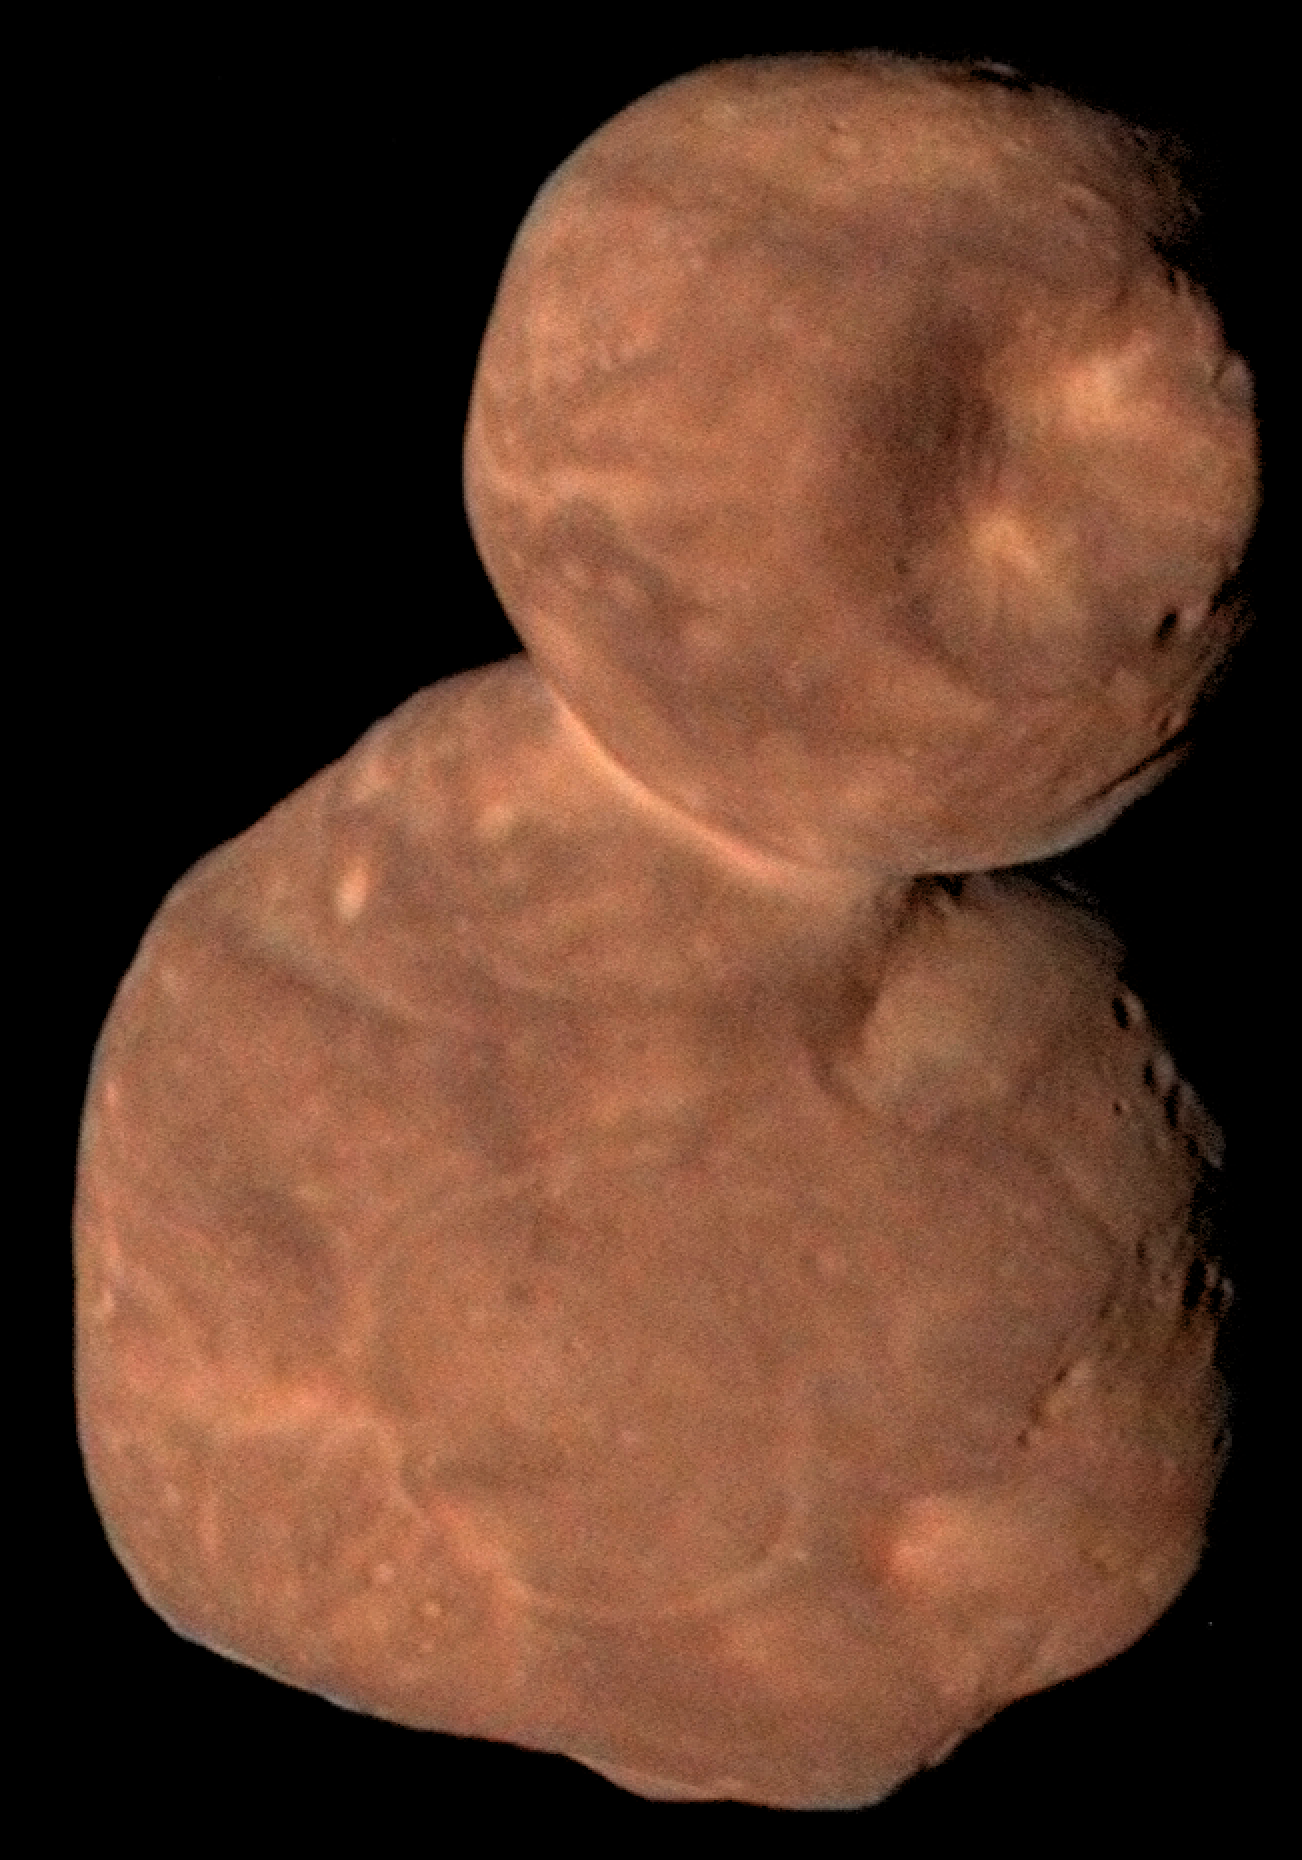
\includegraphics[width=0.45\textwidth]{mu69-named-arrokoth.png}
\caption{\textbf{Short description.} Long description of Arrokoth/MU69. Image taken from \url{https://www.nasa.gov/feature/far-far-away-in-the-sky-new-horizons-kuiper-belt-flyby-object-officially-named-arrokoth}.
}
\label{fig1}
\end{figure}



\section*{Methods}
\ \\
\noindent\textbf{Target.} Description.\\

\noindent\textbf{Observation and data reduction.} Description.

\bibliography{refs}

\begin{addendum}
\item[Acknowledgements] Description.
\item[Author contributions] Description.
\item[Competing interests] The authors declare no competing interests.
\item[Supplementary information] See the following page(s).
\end{addendum}


\setcounter{figure}{0}
\renewcommand{\figurename}{Supplementary Figure}
\renewcommand{\theHfigure}{\arabic{figure}} 

\begin{figure*}[htb!]
\center
\includegraphics[width=0.9\textwidth]{kuiper-belt.jpeg}
\caption{Description of this supplementary image. Image taken from \url{https://www.nasa.gov/feature/far-far-away-in-the-sky-new-horizons-kuiper-belt-flyby-object-officially-named-arrokoth}}
\label{fig1-sup}
\end{figure*}

 
\end{document}